\section{Introduction}

High-dimensional data poses a challenge to traditional likelihood-based modeling approaches.  Penalized regression is an increasingly popular method that is well suited to handle high-dimensional data.  An appealing aspect of many penalized approaches is that they yield sparse models where only a subset of the available variables are ``selected'' by the model in the sense of having non-zero coefficient estimates.  The number of variables in the selected subset can be controlled by changing the degree of penalization, making penalized regression an attractive tool for variable selection in the high-dimensional setting.

Perhaps most popular of these penalized approaches is the least absolute shrinkage and selection operator (lasso) introduced by \citet{tibshirani_1996}. The lasso imposes a penalty on the L1 norm of the estimated regression coefficients that is governed by a single parameter, $\lambda$, such that larger values of $\lambda$ result in more sparse models. In this paper we focus on the variables that are selected by a penalized regression model, in particular we examine how certain are we that these selections are not false discoveries. We do this under the general setting of likelihood-based penalized regression models, which includes GLM and Cox Proportional Hazards models under many popular penalties, including the lasso, SCAD \citep{SCAD}, MCP \citep{MCP}, and elastic net \citep{Elastic_Net}.

To address this question of selection reliability, Breheny (2016) originally proposed a method to estimate marginal false discovery rates for linear lasso regression. Here we begin by outlining this approach, then we extend it to a more general class of regression models.  After doing so, we will compare our estimator's performance with other approaches that are commonly used in high dimensional variable selection.  We conclude by applying our approach to two case studies involving high-dimensional survival and high-dimensional classification data to demonstrate the estimator's practical utility.

\section{Marginal False Discovery Rates}

False discoveries are straightforward to define when conducting single variable hypothesis tests; a false discovery is a significant result that is actually independent of the outcome. In the regression framework, where many variables are being considered simultaneously, the idea of a false discovery becomes complicated. A standard approach, which we refer to as the \textit{fully conditional} perspective, is to consider a feature $X_j$ to be a false discovery if it is independent of the outcome conditional upon all other features, ie: $X_j \independent Y | X_{k \neq j}$. Many penalized likelihood methods result in only a subset of the available variables being active in the model, thereby making fully conditional inference difficult. This motivates the \textit{pathwise conditional} perspective, which considers the model where variable $j$ first becomes active and conditions only on the other variables present in the model at that time when assessing whether or not variable $j$ is a false discovery.

\begin{figure}[!htb]
\centering
\begin{tikzpicture}[node distance=1cm]

% nodes %
\node(b)[text centered] {$B$};
\node(u)[below of = b, text centered] {$ $};
\node(a)[left of = u,  text centered, xshift = -1.5cm] {$A$};
\node(c)[right of = u, text centered, xshift = 1.5cm] {$C$};
\node(y)[below of = u, text centered] {$Y$};
 
% edges %
\draw [arrow] (a) -- (b);
\draw [arrow] (a) -- (y);

\end{tikzpicture} \\
\caption{\label{Fig:diagram} Causal diagram showing three types of relationships between variables and the outcome.}
\end{figure}

In this paper we adopt a weaker \textit{marginal false discovery} definition which we motivate using the causal diagram depicted in Figure~\ref{Fig:diagram}. In this diagram variable $A$ has a direct causal relationship with the outcome variable $Y$ and should never be considered a false discovery. Variable $C$ is independent of variable $Y$ regardless of any variables we adjust for and should always be considered a false discovery. 

Variable $B$ is is correlated with variable $Y$, but after adjusting for $A$ it is independent of $Y$. Depending upon the perspective taken, $B$ might or might not be considered a false discovery. In a fully conditional approach $B$ should always considered a false discovery, however in a pathwise approach this depends upon whether $A$ is active in the model. Further complicating things is the identifiability problem inherent in distinguishing whether $A$ or $B$ is the variable driving changes in $Y$. Our approach avoids these complications by only considering variables like $C$ to be marginal false discoveries, a definition consistent with univariate testing. Regardless of the perspective taken on variables like $B$, it remains that identifying marginal false discoveries provides a useful way of assessing how many variables in a model are purely noise.   

\subsection{Penalized Likelihood Optimization}

Consider data of the usual form $(\y, \X)$, where $\y$ denotes the response variable(s) for $i = \{1, \ldots, n\}$ independent observations, and $\X$ is a matrix containing the values of $j = \{1, \ldots, p\}$ explanatory variables such that entry $x_{i,j}$ corresponds to the value of the $j^{\textrm{th}}$ variable for the $i^{\textrm{th}}$ observation.  We assume the columns of $\X$ are standardized such that each variable has a mean of $0$ and $\sum_i \x_j^2 = n$.

The explanatory variables in $\X$ are related to $\y$ through a probability model involving coefficients $\bb$.  The fit of the model to the data can be summarized using the log-likelihood, which we denote $\ell(\bb|X,\y)$.  In the classical setting, $\bb$ is estimated by maximizing $l(\bb|X,\y)$.  However, this approach is unstable in high dimensions unless an appropriate penalty, denoted $P_{\lambda}(\bb)$, is imposed on the size of $\bb$.
In this case, $\bbh$ is found by minimizing the objective function

\al{eq:obj}{
  Q(\bb|X,\y) =  -\frac{1}{n} \ell(\bb|X,\y) + P_{\lambda} (\bb).
}

In the classical setting, the maximum likelihood estimate is found by setting the score, $\u(\bb) = \nabla \ell(\bb|X,\y)$, equal to zero.  The penalized maximum likelihood estimate, $\bbh$, is found similarly, although allowances must be made for the fact that the penalty function is typically not differentiable.  These penalized score equations are known as the Karush-Kuhn-Tucker (KKT) conditions in the convex optimization literature, and are both necessary and sufficient for a solution $\bbh$ to minimize $Q(\bb|X,\y)$.

In a likelihood-based regression model, the likelihood depends on $\X$ and $\bb$ through a linear predictor $\be = \X\bb$; in other words, we can equivalently express the likelihood in terms of a loss function $f(\be|\y)=-\ell(\bb|\X,\y)$.
In what follows, we assume that the loss function is strictly convex with respect to the linear predictors $\be$; note that this does not imply strict convexity with respect to $\bb$.
Under these conditions, any solution $\bbh$ that minimizes \eqref{eq:obj} with the lasso penalty $P_{\lambda} (\bb) = \lambda||\bb||_1$ must satisfy \citep{lasso_kkt}:
\begin{alignat*}{2}
  \tfrac{1}{n}u_j(\bbh) &= \lam \textrm{ sign}(\hat{\beta}_j) &\quad \text{if } \hat{\beta}_j &\neq 0 \\
  \tfrac{1}{n}u_j(\bbh) &\in [-\lam,\lam]  &\quad \text{if }  \hat{\beta}_j &= 0
\end{alignat*}
for $j \in \{1, \ldots, p\}$.

%In penalized regression framework $f(X\bb) =  -\frac{1}{n}l(\be|X,\y)$ and $ \nabla f(X\bbh) = -\frac{1}{n} u(\beh)$, where $u$ is the unpenalized score function with respect to $\be$.

\subsection{Estimation of mFDR}

In this section, we use classical distributional properties of the score function along with the KKT conditions given above to derive an estimator for the number of marginal false discoveries in the lasso model.
The basic intuition behind the derivation is that, given certain regularity conditions, if feature $j$ is a marginally independent of $\y$, then $Pr(\bh_j \neq 0)$ is approximately equal to $Pr(\tfrac{1}{n}\abs{u_j(\bb)} > \lam)$, where the classical score statistic $\u$ is evaluated at the true value of $\bb$ provided that the log-likelihood is correctly specified (i.e., that the model assumptions hold).
Given this result, the asymptotic normality of the score allows us to estimate this tail probability, and with it, the expected number of marginal false discoveries at a given value of $\lam$.

Three regularity conditions are required for these theoretical results to hold.  These are given below, where we let $\W = \nabla^2f$ denote the $n \times n$ matrix of second derivatives of the loss function with respect to $\be$, such that the classical Hessian matrix $\nabla^2 \ell (\bb) = -\X^T\W\X$.  We use $\W$ to denote this matrix evaluated at the true value of $\bb$ and $\hat{\W}$ if evaluated at the lasso estimate.  In addition, we let $v_j=\x_j^T\W\x_j$, with $\hat{v}_j$ defined similarly.

\begin{itemize}
\item (A1) Asymptotic normality of the score function: $(\X^T\W\X)^{-1/2}\u(\bb) \inD N(\zero,  \I)$, where $\I$ denotes the $p \times p$ identity matrix.
\item (A2) Vanishing correlation between noise variables: $\frac{1}{n}\x_j^T\W\X_{-j} \inP \zero$.
\item (A3) Estimation consistency: $\sqrt{n}(\bbh-  \bb)$ is bounded in probability.
\end{itemize}

We can now formally state our main theoretical result.  In interpreting this result, it is important to keep in mind that only features that are marginally independent of the outcome will satisfy both assumption (A2) and $\beta_j=0$.
In other words, the theorem applies to variables like $C$ in Figure~\ref{Fig:diagram}, but not variable $B$: although the regression coefficient for $B$ is zero, its correlation with $A$ violates (A2).

\begin{theorem}
  \label{Thm:main}
  For any solution $\bbh$ of the lasso-penalized objective \eqref{eq:obj}, we have $\bh_j \neq 0$ if and only if
  \as{\tfrac{1}{n}\abs{u_j(\bbh) + v_j\bh_j} > \lam.}
  Furthermore, provided that that (A1)-(A3) are satisfied and $\beta_j=0$,
  \as{\frac{u_j(\bbh) + v_j \bh_j}{\sqrt{v_j}} \inD N(0, 1).}
	%\as{\sqrt{n}\frac{\tfrac{1}{n}u_j(\bbh) + v_j \bh_j}{\sqrt{v_j}} \inD N(0, 1).}
\end{theorem}


\begin{proof}
  The first remark follows directly from the KKT conditions and the fact that, if the loss function is strictly convex, then $\W$ is positive definite and $v_j$ is positive.  The asymptotic normality of the score function (A1) implies that the following Taylor series expansion holds:
\as{\u(\bbh) = \u(\bb) - \X^T\W\X(\bbh - \bb) + o_p(n)(\bbh-\bb).}
Since $\beta_j=0$, we then have
\as{u_j(\bbh) &= u_j(\bb) - \x_j^T\W\X_{-j}(\bbh_{-j} - \bb_{-j}) - \x_j^T\W\x_j\bh_j + o_p(n)\bh_j,\\
\intertext{or}
\tfrac{u_j(\bbh) + v_j \bh_j}{\sqrt{v_j}}  &= \tfrac{u_j(\bb)}{\sqrt{v_j}} - \sqrt{\tfrac{n}{v_j}}[\tfrac{1}{n}\x_j^T\W\X_{-j}][\sqrt{n}(\bbh_{-j} - \bb_{-j})] + o_p(1)\sqrt{\tfrac{n}{v_j}}\sqrt{n}\bh_j.}
%\tfrac{1}{\sqrt{n}}u_j(\bbh) + \sqrt{n}v_j\bh_j &= \tfrac{1}{\sqrt{n}}u_j(\bb) - [\tfrac{1}{n}\x_j^T\W\X_{-j}][\sqrt{n}(\bbh_{-j} - \bb_{-j})] + o_p(1)\sqrt{n}\bh_j.}
The first term converges to $N(0,1)$ by (A1), the second term goes to zero by conditions (A2) and (A3), and the third term also goes to zero by (A3).
\end{proof}

Theorem~\ref{Thm:main} therefore implies that the probability that feature $j$ is selected, given that it is marginally independent of the outcome, is approximately the probability that a random variable following a $N(0, v_j/n^2)$ distribution exceeds $\lam$ in absolute value.
In principle, the expected number of marginal false selections could be obtained by summing this probability over the set of marginally independent noise variables; in practice, since the identity of this set is unknown, a conservative alternative is to sum over all $p$ variables.
This gives the following estimators for the number and rate of marginal false discoveries:
\al{eq:mfdr}{
  \widehat{FD} &= 2 \sum_{j=1}^{p} \Phi \left(\frac{-n\lam}{\sqrt{\hat{v}_j}}\right)\\
  \widehat{mFDR} &= \frac{\widehat{FD}}{|S|},
}
where $S$ is the set of selected variables and $|S|$ its size.

Mention something about upper bound?

\subsection{The mFDR Estimator (OLD)}

TEMPORARILY LEAVING THIS SECTION AROUND FOR COMPARISON

Suppose variable $j$ is a noise variable unrelated to $\y$ marginally, as depicted in Figure~\ref{Fig:diagram}. For a given value of $\lambda$ we use the KKT conditions to describe the probability that variable $j$ is selected by the lasso regression model.

Let $\u(\bb) = \X^T \s(\be)$ denote the unpenalized score function with respect to $\bb$.  To proceed we require the following primary assumptions:

\begin{itemize}
\item A1: Asymptotic normality of the score function: $u(\bb) \xrightarrow{d} N(\zero,  E\big[l''(\bb)\big])$
\item A2: Vanishing correlation between noise variables: $\frac{1}{n}\x_j^T u'(\be)X_{-j} \rightarrow 0$
\item A3: Estimation consistency: $\sqrt{n}(\bbh-  \bb)$ is bounded in probability and $\W = \nabla^2 f(\beh)$ is a consistent estimator of $-E\big[\nabla^2 f(\be)\big]$
\end{itemize}

\noindent{\textbf{Theorem}:} Provided these conditions are met:

\begin{equation}
Pr(\bh_j \neq 0)  \rightarrow Pr\big(\frac{1}{n}|\x_{j}^T \u(\be)| > \lambda\big)
\end{equation}

\begin{equation}
\frac{1}{\sqrt{n}}\x_{j}^T u(\be) \rightarrow N\big(0, V\big) 
\text{   where } V = \lim_{n \to \infty} \tfrac{1}{n}\x_{j}^T \W \x_{j}
\end{equation}

Which together imply:

\begin{equation}
Pr(\bh_j \neq 0)  = 2\Phi \bigg( \frac{-n\lambda}{\sqrt{ \x_j^TW\x_j}} \bigg)
\end{equation}

Where $\Phi$ represents the standard normal cumulative density function.

\noindent{\textbf{Corollary}:}

Using this result to estimate the expected number of marginal false selections simply requires summing over the set of noise variables, however in practice the identity of these variables is unknown. Instead summing over all $p$ variables provides a conservative upper bound and leads to the following:

\begin{align}
&\widehat{FD} = 2 \sum_{j=1}^{p} \Phi \bigg( \frac{-n\lambda}{\sqrt{\x_j^T W \x_j}} \bigg) & \widehat{mFDR} = \frac{\widehat{FD}}{|S|}
\end{align}

The estimated marginal false discovery rate, $\widehat{mFDR}$ is defined to be the ratio of estimated false selections to $|S|$, the total number of variables selected by the lasso model.

\begin{proof}

We begin with the KKT conditions required for the selection of variable $j$.  These conditions directly imply:

\begin{equation*}
Pr(\hat{\beta}_j \neq 0)  = Pr\big(\frac{1}{n}|\x_{j}^T u(\beh)| = \lambda\big)  = Pr\big(\frac{1}{n}|u(\bbh)_j| = \lambda\big)
\end{equation*}

Next we approximate $u(\bbh)$ using a first order Taylor Series expansion centered at $\bb$:

\begin{equation*}
u(\bbh) \sim u(\bb) + u'(\bb)( \bbh - \bb) 
\end{equation*}

\begin{equation*}
\implies \x_j^T \s(\beh) \sim \x_j^T \s(\be) +  \x_j^T f''(\be) ( \beh - \be)
\end{equation*}

This leads to the selection requirement being approximately equivalent to:

\begin{equation*}
\frac{1}{n}|\x_j^T \big( \s(\be) + f''(\be) (\beh - \be)  \big) | = \lambda
\end{equation*}

Because variable $j$ is unrelated to the outcome $\be= X_{-j}\bb_{-j}$.  Additionally we separate $\beh$ into $X_{-j}\bbh_{-j} + \x_j^T\beta_j$ leading to the following expression for the selection requirement:

\begin{equation*}
\frac{1}{n}|\x_j^T \s(\be) + \x_j^T f''(\be)X_{-j}(\bbh_{-j} -  \bb_{-j}) + \x_j^T f''(\be)\x_j \hat{\beta}_j |  = \lambda
\end{equation*}

Because sign$(\bh_j) =$ sign$(\x_j^T \s(\be))$ the selection requirement can be expressed by the inequality:

\begin{equation*}
\frac{1}{n}|\x_j^T  \s(\be) + \x_j^T f''(\be)X_{-j}(\bbh_{-j} -  \bb_{-j}) |  \geq \lambda
\end{equation*}

Assumptions A2 and A3 imply:

\begin{equation*}
\frac{1}{n}\x_j^T f''(\be)X_{-j}\sqrt{n}(\bbh_{-j} -  \bb_{-j})  \rightarrow 0
\end{equation*}

Thus we have arrived at (1).  Assumption A1 leads directly to the distributional result in (2) which in turn leads directly to the estimators in (4).\qedhere

\end{proof}
  
\subsection{Other Penalty Functions}

The KKT conditions are necessitated by the use of a non-differentiable penalty function. While the lasso penalty is one example of this, many other non-differentiable penalties exist and often have KKT conditions very similar to those of the lasso. This similarity allows the mFDR estimator to be easily adapted to these penalty functions. As an example we consider the elastic net \citep{Elastic_Net}, which utilizes two penalty parameters $\lambda_1, \lambda_2$. The elastic net solution is found by minimizing $-\frac{1}{n} \ell(\bb|X,\y) + \lambda_1 ||\bb||_1 + \frac{\lambda_2}{2}||\bb||_{2}^2 $. The KKT conditions of elastic net dictate that for $\hat{\beta_j} \neq 0$:

\begin{equation*}
\frac{1}{n}\x_{j}^T u_j(\bbh) = \lambda_1 sign(\hat{\beta}_j) + \lambda_2 \hat{\beta}_j
\end{equation*}

Compared with the lasso, only the right hand side of the selection condition has changed. Because $\lambda_1 + \lambda_2|\hat{\beta}_j| \geq \lambda_1$ the same inequality that we derived to express feature selection by the lasso also applies to the elastic net, allowing for an identical mFDR estimator to be used. Other notable penalties which result in the same estimator are the minimax concave penalty (MCP) introduced by \citet{MCP} and the smoothly clipped absolute deviations (SCAD) penalty introduced by \citet{SCAD}. Both MCP and SCAD are non-convex penalties that produce sparse estimates like the lasso, but they have the benefit of relaxing the degree of penalization on variables with large effects. This leads to solutions with greater sparsity and less biased coefficient estimates. We note that while many penalties will lead to the same estimator asymptotically, the exact conditions required to achieve (A3) will differ. This can be seen in simulation studies presented later in the paper, which include results for both the lasso and MCP penalties.

\subsection{Logistic Regression}

So far we have presented the mFDR estimator in the general setting of penalized likelihood optimization. One specific scenario where the estimator can be applied is penalized logistic regression. Suppose $y_i$ follows a Bernoulli distribution with success probability $\pi_i$. In logistic regression the logit of $\pi_i$ is modeled as a function of $\be = X\bb$, which results in a likelihood consisting of the product of $n$ independent Bernoulli distributions with parameters $\pi_i = \frac{\exp(\eta_i)} {1 + \exp(\eta_i)}$.

%\begin{equation*}
%L(\be) = \prod_{i=1}^{n} \pi_i^{y_i} (1 - \pi_i)^{1 - y_i}
%\end{equation*}

Provided the log-likelihood is a convex function of $X\bb$, which clearly applies to logistic regression, the mFDR estimator depends on the likelihood via the structure of $\W$, which is needed to calculate $\hat{v}_j$. For logistic regression $\W$ is a diagonal matrix with the $i^{th}$ diagonal element given by $\pi_i(1 - \pi_i)$. We estimate $\hat{\pi}_i = \frac{\exp(\x_i^T\hat{\bb})} {1 +\exp(\x_i^T\hat{\bb})}$ which by (A3) leads to a consistent estimator of $v_j$.

\subsection{Cox Regression}

Another setting where mFDR can be used is penalized Cox regression. Here the outcome of interest contains two components, a time, $y_i$, along with an accompanying indicator variable, $d_i$, where $d_i = 1$ indicates $y_i$ is an observed event time and $d_i = 0$ indicates $y_i$ is a right censoring time.  

Let $t_1 < t_2 < \ldots < t_m$ be an increasing list of unique failure times indexed by $k$. The Cox model assumes a semi-parametric form of the hazard such that $h_i(t) = h_0(t)e^{\x_i^T \bb}$, where $h_i(t)$ is the hazard for observation $i$ at time $t$ and $h_0(t)$ is a common baseline hazard. Cox regression is based upon the Cox partial likelihood \citep{Cox1972}:

\begin{equation*}
L(\be)  = \prod_{k=1}^{m} \frac{\exp(\be_k)}{\sum_{r \in R_k} \exp(\be_r) } 
% \prod_{k=1}^{m} \frac{\exp(\x_k^T\bb)}{\sum_{r \in R_k} \exp(\x_r^T\bb) } 
\end{equation*}

Because the partial likelihood is a convex function of $X\bb$, the KKT conditions described in Section 2.2 apply in the same way which they applied to the full likelihood in the logistic regression case. Although when estimating mFDR an additional consideration is necessary for (A2) to hold, here we also require noise variables be uncorrelated with each other with respect to their influence on the censoring mechanism. This additional requirement is needed because when a variable is related to the censoring mechanism its distribution will drift over time as certain values are disproportionately removed from the risk set, which can induce to correlations between the noise variables that would otherwise be uncorrelated. The impact of this additional concern on the $\widehat{mFDR}$ is further assessed via simulation in section 3.3. 

As with penalized logistic regression, the mFDR estimator for penalized Cox regression depends on the likelihood through $\W$. In Cox regression the form of $\W$ is considerably more complicated due to the non-diagonal elements being non-zero. Motivated by the arguments in \citet{Simon_COXPH_CD} we simplify our estimate of $v_j$ by taking the off-diagonal elements of $\W$ to be zero in order to greatly improve computational efficiency. In simulations we found no difference the accuracy of $\widehat{mFDR}$ when using the diagonal approximation of $\W$ in place of the full matrix.

\section{Simulations}

In this section we study the behavior of the mFDR estimator via several simulation studies. In each study we generate $j \in \{1, \ldots, p\}$ variables from standard normal distributions for $i = 1, \ldots, n$ subjects. We consider three different penalized likelihood models, logistic regression, Cox regression, and linear regression.

For logistic regression scenarios, binary outcomes are generated from independent Bernoulli distributions with parameter $\pi_i = \frac{\exp(\x_i^T \bb)} {1 + \exp(\x_i^T \bb)}$. For Cox regression scenarios, survival outcomes are generated from independent exponential distributions with rate parameter $\theta_i = \exp(\x_i^T \bb)$. And for linear regression scenarios outcomes are generated from the model $y_i = \x_i\bb + N(0,\sigma^2)$. Factors including $p$, $n$, and $\bb$, the correlation between variables, and censoring are varied throughout these simulations.

\subsection{Inaccuracy, Sample Size, and Correlation}

Potential inaccuracy of $\widehat{mFDR}$ arises from two places, first by using the asymptotic distribution of the score function, and second in the convergence of the remainder term to zero. Consequently we study at the effect of two factors, sample size, which will impact both of sources of inaccuracy, and correlation between noise variables, which impacts the remainder term, on accuracy. We evaluate accuracy by comparing $\widehat{mFDR}$ with the observed proportion of noise variables at each value of a fixed $\lambda$ sequence averaged across 1,000 simulation iterations.

We generate our data using $p = 40$ with $\beta_{1:4} = \frac{10}{\sqrt{n}}$ and $\beta_{5:40} = 0$ while varying $n$ from 100 to 1,000 in increments of 100. We take $\bb$ to be function of $n$ in order to maintain the difficulty of the variable selection problem as $n$ increases.  Without this provision, when $n$ is large, all of the true variables are easily selected very early in the $\lambda$ sequence and false selections are extremely rare until the very end of $\lambda$ sequence where they occur rapidly, leading to the observed proportion of false selections at a given $\lambda$ being very unstable.

In total we assess twelve different scenarios consisting of each possible combination of:
\begin{itemize}
\item Two different correlation structures: independent noise variables and correlated noise variables
\item Three different regression methods: linear regression, logistic regression, and Cox regression
\item Two different penalties: lasso and MCP. 
\end{itemize}
For our correlated setting noise variables are given an autoregressive correlation structure based upon their index such that $Cor(\x_j,\x_k) = 0.8^{|j - k|}$. We display the average estimated mFDR at the $\lambda$ value where the average observed proportion of noise variables is 10\%.

\begin{figure} [!htb]
 \centering
  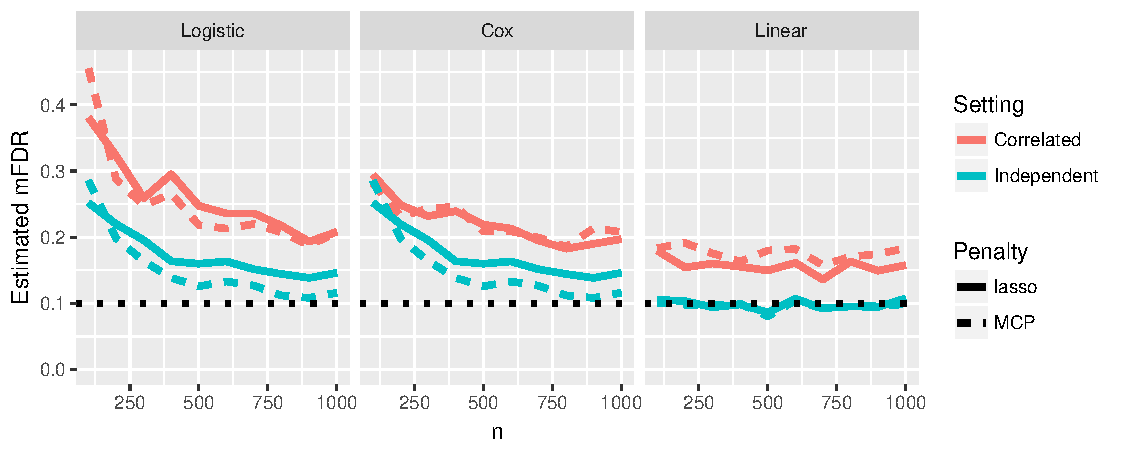
\includegraphics[width=.9\textwidth]{ggconverge3.pdf}
  \caption{Inaccuracy of the mFDR estimator}
\end{figure}

The mFDR estimator tends to be conservative with the degree of conservatism decreasing as $n$ increases. In the case of independent noise variables the estimator approaches the nominal marginal false discovery rate as $n$ increases. The convergence occurs nearly instantaneously linear regression, with the estimator being very accurate even at $n=100$, and more slowly for logistic and Cox regression with the estimator remaining very slightly conservative even when $n > 500$. The MCP penalty leads to faster convergence and better accuracy than the lasso penalty, this is particularly noticeable in the logistic and Cox regression settings. The improvement is likely due to the MCP's tendency towards less biased coefficient estimates which results in more accurate estimates of $v_j$ and also faster convergence of the remainder term.

The correlated setting induces a noticeable conservative bias that is cannot be resolved by increasing the sample size. This issue is not unique to mFDR as many methods for controlling false discovery rates also tend to be conservative in correlated settings. Even with its conservative nature, mFDR can still be useful tool in assessing the reliability of selections made by a penalized regression model by providing an upper bound on the proportion of false selections in cases of moderate correlation.

\subsection{Inaccuracy and Censoring}

An additional concern arises in the Cox regression setting due to censoring.  We assess the influence of variable associations with the censoring mechanism by comparing two scenarios. In each scenario censoring times are generated from exponential distributions with $\theta_{i} = \exp(\x_i^T \bg)$, and in scenario A four noise variables are related to censoring via $\bg_A = (0, 0, 0, 0, 1, -1, 1, -1, 0, \ldots, 0) $; while in scenario B all variables are independent of censoring with $\bg_B = (0, \ldots, 0))$. By design, each of these scenarios, on average, results in 50\% of the observations being censored.  The same set of $n = 100$ true failure times is used for both scenarios and are generated from independent exponential distributions with rate parameter $\theta_i = \exp(\x_i^T \bb)$, where $\beta_{1:4} = 1$ and $\beta_{5:40} = 0$.
\begin{table}[!htb]
 \caption{Average true mFDR (10,000 simulations) when the estimated mFDR is 10\%}
\centering
\begin{tabular}{c | c c}
  \hline
 Scenario & lasso & MCP   \\  [0.5ex]
  \hline 
   A & 1.02\% & 6.72\% \\ 
   B &  1.33\% & 7.31\% \\ 
   \hline
\end{tabular}
\end{table}

The correlation induced between noise variables induced by their relationship with censoring in scenario A leads to a slightly more conservative mFDR estimator. The degree of conservatism is minor in comparison to the effects of sample size and correlation between noise variables with respect to the outcome.

\subsection{Comparison with Other Methods}

In this simulation study we assess different methods of variable selection used in the high-dimensional setting. We generate our data based upon the structure depicted in Figure~\ref{Fig:diagram}, we use $n = 400$ and $p = 1000$ with ten variables are causally related to the outcome, like ``A", such that $\beta_{1:10} = b$ and vary $b$ throughout the study. Corresponding to each causal variable we generate nine correlated ($\rho = 0.5$) variables, akin to ``B". The remaining 900 variables are noise, akin to ``C", however they are correlated with each other such that $Cor(\x_j,\x_k) = 0.8^{|j - k|}$, thereby creating a situation where the mFDR estimator will be conservative.

We assess the average number of selections for each variable type (``A", ``B", ``C") after applying each of the following methods:
\begin{itemize}
\item Our mFDR approach, where variables are selected by the lasso using the smallest $\lambda$ with $\widehat{mFDR} \leq .1$.  
\item A sample splitting approach, motivated by \citet{Sample_Splitting}, where we first fit a lasso regression model on half of the data to select the top 20 variables. We then use the remaining data to fit a unpenalized regression model on the variables selected in the first stage. With the unpenalized model we conduct traditional hypothesis tests on the regression coefficients and apply the Benjamini-Hochberg procedure \citep{BH_1995} to control the false discovery rate at $10\%$. We mandate that only 20 variables are selected in the first stage so that the second stage model contains 10 events per variable \citep{peduzzi_epv}.
\item The covariance testing approach \citep{CovTest}, which we use in conjunction with the forward stopping rules proposed by \citet{GSell2016} to control the pathwise false discovery rate at $10\%$. 
\item A large scale univariate testing approach which fits an unpenalized regression model to each variable individually, conducts a hypothesis test on the variable coefficient, and then adjusts the resulting p-values using the Benjamini-Hochberg procedure to control the false discovery rate at $10\%$.
\item A lasso approach which uses 10-fold cross validation to select the $\lambda$ and makes no attempt to control the false discovery rate.
\end{itemize}

\begin{figure} [!htb]
 \centering
  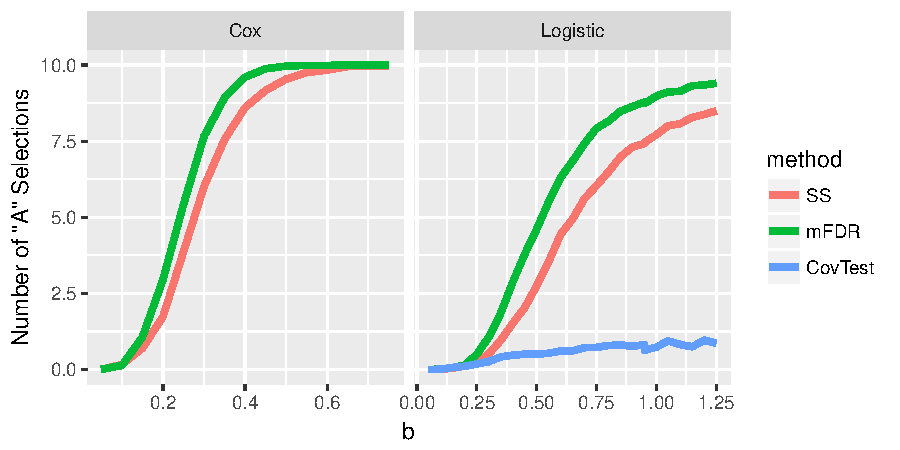
\includegraphics[width=0.75\textwidth]{ggpower.pdf}
  \caption{\label{Fig:lassopower} The number of true, ``A", variables selected by each lasso based method of false discovery rate control, averaged across 1,000 simulation iterations plotted as a function of $\beta$.}
\end{figure}

Compared to the other false discovery rate control methods which use penalized regression, the mFDR approach selects more causally important variables at every value of $b$. This result comes with the caveat that despite being available in the ``CovTest" package, the covariance test for logistic regression is currently considered to be experimental by the package creators. The test has not yet been implemented in the package for Cox regression. 

\begin{figure} [!htb]
 \centering
  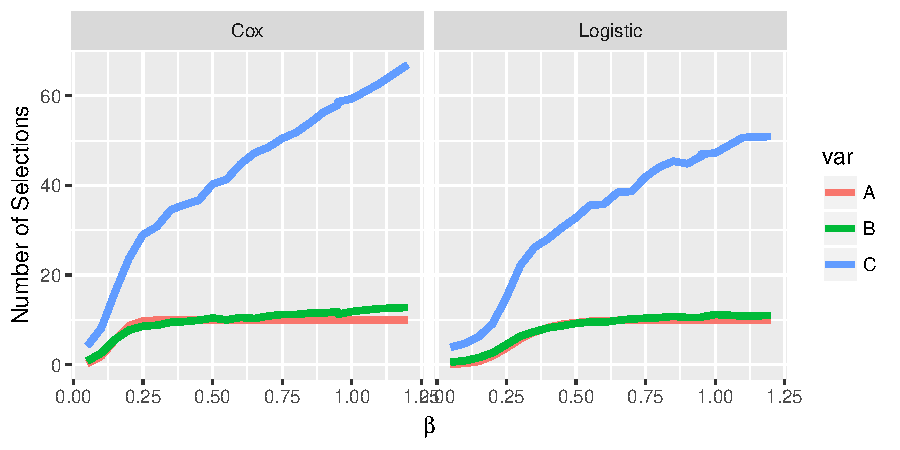
\includegraphics[width=0.75\textwidth]{ggcv.pdf}
  \caption{The average number of selections for each type of variable depicted in Figure~\ref{Fig:diagram} is plotted for cross validation as function of $\beta$ }
\end{figure}

Cross validation is the most effective in selecting true variables, however it does not control number of false selections. In fact it selects more and more noise variables as the $\beta$ increases. While all of the other approaches resulted in false discovery rates well under 10\% throughout our simulations, as many as $80\%$ of the selections made by cross validation were noise variables for larger values of $\beta$. This is particularly troublesome since these additional noise variable selections offer no advantage when it comes to selecting true variables in this scenario, thus highlighting a major difference between using the lasso for prediction and using the lasso for variable selection.

\begin{figure} [!htb]
 \centering
  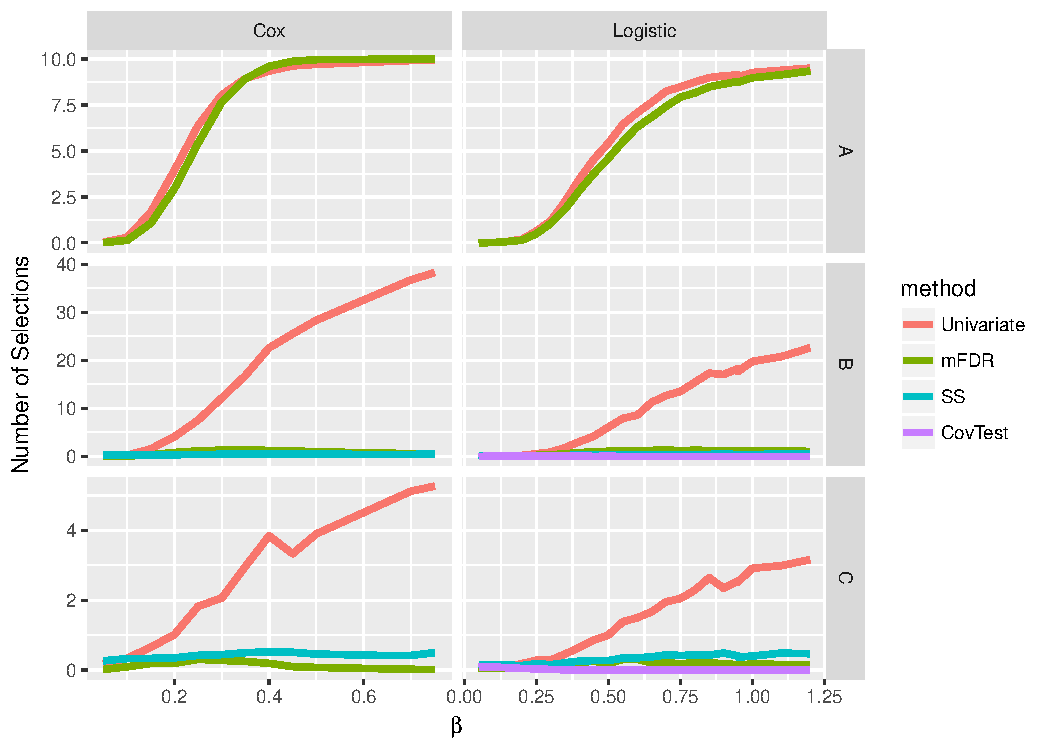
\includegraphics[width=0.75\textwidth]{ggunivariate.pdf}
  \caption{The average number of selections, for each type of variable depicted in Figure~\ref{Fig:diagram}, is plotted as function of $\beta$ for each method which controls the false discovery rate.}
\end{figure}

The mFDR and univariate approaches are both designed to control the proportion of marginal false discoveries without making any claims pertaining to correlated, ``B", variables. The two methods each select causally important variables at a comparable rate, however mFDR has a distinct advantage when it comes to reducing the number of correlated selections. The mFDR approach even does as well at limiting correlated variable selections as the sample splitting and covariance approaches which are based upon fully conditional and pathwise conditional false discovery definitions respectively. 

\begin{table}[ht]
\centering
\begin{tabular}{c | r r r r}
  \hline
 $\beta$ & univariate (Cox) & mFDR (Cox) & univariate (Logistic) & mFDR (Logistic) \\ 
  \hline
  0.25 & 3.50 & 17.68 & 2.31 & 3.26 \\ 
  0.35 & 3.01 & 36.20 & 4.94 & 11.10 \\ 
  0.45 & 2.89 & 102.21 & 5.31 & 15.34 \\ 
  0.65 & 2.38 & 333.33 & 4.59 & 32.59 \\ 
  0.75 & 1.89 & 750.00 & 4.15 & 47.56 \\ 
   \hline
\end{tabular}
\caption{The ratio of A:C variable selections for various values of $\beta$.}
\end{table}

In practice it can be difficult to distinguish variables like ``A" from variables like ``B", but the redundant selection of both comes with the unfortunate consequence of allowing more noise variables to be selected. This can be seen with univariate testing, which selects many correlated variables and consequently also selects a greater absolute number of noise variables than the other methods. So while both the mFDR and univariate approaches use the same false discovery definition and tend to select a similar amount true variables, the univariate approach does so while often selecting many more correlated and noise variables. For the univariate approach, this allows the rate of true variable selections per noise variable selection to remain relatively low, and even decrease, as $\beta$ increases. In contrast, with the mFDR approach, the true variable to noise variable selection rate increases with $\beta$.  

\section{Case Studies}

\subsection{Lung Cancer Survival and Gene Expression}
\citet{Shedden2008} studied the survival of 442 early-stage lung cancer subjects. Researchers collected high-dimensional gene expression data consisting of 22,283 genetic features and additional clinical covariates of age, race, gender, smoking history, cancer grade, and whether or not the subject received adjuvent chemotherapy.  

In our analysis we aim to select of important genetic features while controlling the marginal false discovery rate.  We use a penalized Cox Proportional Hazards regression model that allows for all of the clinical covariates to enter the model unpenalized while using the sparsity introduced by penalization to select additional genetic features.  We target an mFDR of 10\% and explore both the lasso and MCP penalties, while comparing our results to those of other methods.

\begin{figure} [!htb]
 \centering
  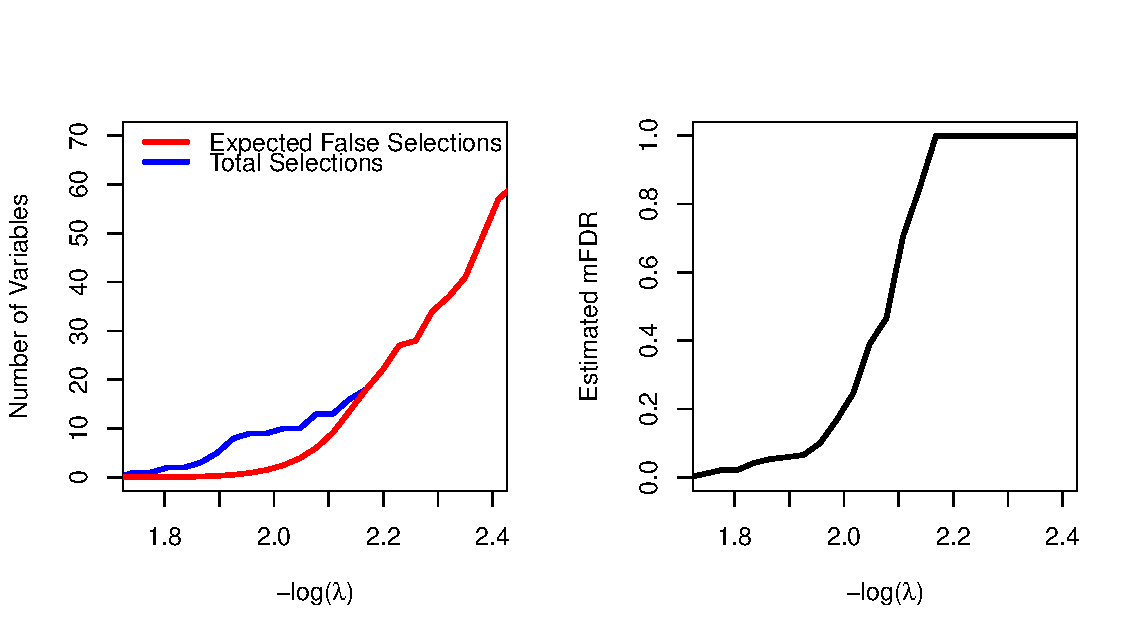
\includegraphics[scale = .7]{Shedden.pdf}
  \caption{\label{Fig:Shedden} The estimated mFDR compared to the total number of features selected and how many expected false selections were made at each $\lambda$ value}
\end{figure}

In Figure~\ref{Fig:Shedden} we see a discrepancy between the total number of selections and the expected number of false selections for many values of $\lambda$, this indicates that some of the genetic features in the dataset are likely to be truly related to survival. 

Using a target 10\% mFDR leads to a choice of $\lambda$ that selects, 9 genetic features when using the lasso penalty. Using cross validation results in the selection of a much smaller $\lambda$ which corresponds to the selection of 28 genetic features however the estimated mFDR at this choice of $\lambda$ is 100\% indicating that many of these selections are likely to be noise variables. Using the MCP penalty, the targeted 10\% mFDR threshold results in the selection of only 2 genetic features and cross validation selects 26 genetic features. This is reflective of the tendency of the MCP penalty to lead to more parsimonious models.

For comparison we analyze the data using the approach proposed by \citet{Meinshausen2009}, which repeatedly performs sample splitting using a large number random splits. Using this approach we are unable to select any genetic features. Additionally the current version of the covTest package, which is used to carry out the covariance testing approach, currently does not accommodate survival data.

As another comparison we apply a large scale univariate testing approach to the Shedden data in two ways. The first fits a univariate Cox regression model to each genetic feature and tests the features effect on survival.  The second is similar except with each model adjusting for clinical covariates in addition to the single genetic feature.  After using the Benjamini-Hochberg procedure to control the false discovery rate at 10\%, these two univariate testing approaches result in the selection of 862 and 803 features respectively. This is illustrative of the difference between model based approaches and large scale univariate testing. Univariate approaches tends select many features from correlated groups, adding a degree of redundancy to the results. Whereas modeling approaches instead tend to select a single representative from each group of correlated features.  

\subsection{Lung Cancer Status Among Smokers}
\citet{Spira2007} collected RNA expression data from histologically normal bronchial epitheliums of $n = 192$ smokers of which 102 had developed lung cancer and 90 had not developed lung cancer.  We are interested identifying genetic features that are indicative of whether or not a smoker has lung cancer.  For our analysis we a penalized fit logistic regression model using both the lasso and MCP penalties. We compare the results at $\lambda$ values chosen using estimated mFDR, cross validation, and the covariance test as well as the selections made by sample splitting. We also compare these model based approaches to the traditional univariate approach with false discovery rate control.

\begin{table}[ht]
\centering
\begin{tabular}{c|rrr|rrr}
  \hline
 & & lasso & & & MCP & \\
 \hline
$\lambda$ & EF & S & mFDR & EF & S & mFDR \\ 
  \hline
0.2041 & 0.00 &   0 & 0.00 & 0.00 &   0 & 0.00 \\ 
  0.1980 & 0.00 &   2 & 0.00 & 0.00 &   2 & 0.00 \\ 
  0.1921 & 0.00 &   4 & 0.00 & 0.00 &   2 & 0.00 \\ 
  0.1864 & 0.00 &   6 & 0.00 & 0.00 &   3 & 0.00 \\ 
  0.1809 & 0.01 &   6 & 0.00 & 0.01 &   4 & 0.00 \\ 
  0.1755 & 0.02 &   6 & 0.00 & 0.02 &   4 & 0.01 \\ 
  0.1702 & 0.04 &   6 & 0.01 & 0.04 &   4 & 0.01 \\ 
  0.1652 & 0.08 &   8 & 0.01 & 0.08 &   5 & 0.02 \\ 
  0.1602 & 0.15 &   9 & 0.02 & 0.14 &   5 & 0.03 \\ 
  0.1555 & 0.27 &   8 & 0.03 & 0.25 &   5 & 0.05 \\ 
  0.1508 & 0.47 &   8 & 0.06 & 0.42 &   5 & 0.08 \\ 
  0.1463 & 0.78 &  10 & 0.08 & 0.69 &   5 & 0.14 \\ 
  0.1420 & 1.27 &  10 & 0.13 & 1.10 &   5 & 0.22 \\ 
  0.1377 & 2.00 &  11 & 0.18 & 1.72 &   8 & 0.22 \\ 
  0.1336 & 3.10 &  13 & 0.24 & 2.69 &   7 & 0.38 \\ 
   \hline
\end{tabular}
 \caption{The estimated mFDR results for 15 values of the $\lambda$ sequence which straddle our target mFDR}
\end{table}

Using the lasso penalty and a target mFDR threshold of 10\% we choose $\lambda = 0.146$, corresponding to the selection of 10 features.  Cross Validation selects a $\lambda$ of 0.056 corresponding to the selection of 40 features. However the estimated mFDR at the $\lambda$ chosen by cross validation is 100\%, indicating that many of these selections are likely to be noise variables. If instead we use the MCP penalty we select a $\lambda$ value of 0.1508, corresponding to 5 features, when targeting 10\% mFDR; and using cross validation we select a $\lambda$ value of 0.0666, corresponding to 14 features. Once again the estimated mFDR at the $\lambda$ chosen by cross validation is 100\%.  

The sample splitting approach, using 100 random splits, does not select any features after controlling the false discovery rate. Only a single genetic feature reached the second stage in at at least half of the splits but its median p-value was not significant. Similarly the covariance testing approach also does not select any features.  The first variable to enter the model has a p-value of 0.475 and when the ForwardStop procedure is applied we are unable to move beyond the intercept only model without the false discovery rate exceeding 10\%.

As a final comparison, we applied the univariate testing approach to these data in two ways. The first uses t-tests to assess the difference in expression for each genetic feature for the two groups while controlling the false discovery rate at 10\% using the Benjamini$-$Hochberg procedure.  This procedure ends up selecting selecting 2,965 genetic features. The second approach uses univariate logistic regression instead of t-tests, which leads to selection of 2,833 genetic features. The large number of feature selections by both of these univariate approaches again illustrates why a model based approach, which will tend to select a single feature from each correlated group of variables, might be preferable. 

\section{Discussion}
Estimating the marginal false discovery rate of a penalized likelihood model is a useful way of assessing the reliability of a selected set of features. Unlike other approaches that have a similar goal, such as sample splitting or the covariance test, mFDR uses less strict definition of a false discovery which does not condition on any other variables and consequently only limits variables that are strictly noise. The simulation comparisons in this paper demonstrate that while mFDR is based upon a weaker false discovery definition, it can do quite well in limiting the number of correlated, non-causal variable selections.

The mFDR estimator is currently implemented in R in the \text{ncvreg} package \citep{Breheny2011} using the \text{mFDR} function. The function accepts an ncvreg fitted model  and provides estimates for the expected number of false discoveries, as well as the mFDR for each value of the $\lambda$ sequence used in fitting the model. The function accommodates lasso, MCP, SCAD, elastic net, and MNet \citep{Huang2016} penalties and provides a convenient model summary measure for penalized regression models.

We also mention that in the simulations and case studies the sample splitting approach had to be coded manually due to existing software being unable to handle logistic and survival models. The covariance testing approach was implemented using the \text{CovTest} package \citep{CovTest} and the \text{forwardStop} function of the \text{SelectiveInference} package \citep{Selective_Inference}, but is cautioned as being developmental for logistic regression and is not currently implemented for Cox regression. The lack of software that can handle GLM and Cox models adds to the appeal of using mFDR to assess feature selection reliability after fitting penalized regression model with a binary or survival outcome.
